\documentclass[14pt, a4paper, fleqn, twoside]{extreport}

\usepackage[T2A]{fontenc}
\usepackage[utf8]{inputenc}
\usepackage[english,russian]{babel}
\usepackage{url}
%\usepackage{pscyr}

%\renewcommand{\rmdefault}{ftm}
\usepackage{setspace}
\onehalfspacing

\usepackage{changepage}
\usepackage{indentfirst} %первый абзац
%%\usepackage{moreverb}
\usepackage[noend]{algorithmic}
\usepackage{amssymb, amsmath, multicol,amsthm}
%%
\usepackage{enumitem, multicol}
\usepackage{titleps,lipsum}
%%
\usepackage{mathrsfs}
\usepackage{verbatim}
\usepackage{pb-diagram}
\usepackage{graphicx}
\graphicspath{ {images/} }
\usepackage{wrapfig}
\usepackage{xcolor}
\definecolor{new}{RGB}{255,184,92}
\definecolor{news}{RGB}{112,112,112}
\usepackage{wallpaper}
\usepackage{float}
\usepackage{hyperref}
\hypersetup{
%colorlinks=true,%
%linkcolor=news,%
linkbordercolor=new,
}



\usepackage{geometry}
\geometry{top=3.5cm,bottom=2cm,left=2cm,right=2cm}

%\flushbottom
%\ruggedbottom

\binoppenalty=5000
\parindent=0pt

\newcommand{\EDS}{\ensuremath{\mathscr{E}}}
\newcommand*{\hm}[1]{#1\nobreak\discretionary{}%
{\hbox{$\mathsurround=0pt #1$}}{}}
\newcommand{\divisible}{\mathop{\raisebox{-2pt}{\vdots}}}
\renewcommand{\theequation}{\arabic{equation}}
\def\hm#1{#1\nobreak\discretionary{}{\hbox{$#1$}}{}}
\newcommand{\bbskip}{\bigskip \bigskip}



%%\DeclareMathOperator{\tg}{tg}
%%\DeclareMathOperator{\ctg}{ctg}

\let\leq\leqslant
\let\geq\geqslant



% Remove brackets from numbering in List of References
\makeatletter
\renewcommand{\@biblabel}[1]{\quad#1.}
\makeatother
% Header and Footer with logo
\usepackage{lastpage,fancyhdr,graphicx}
\usepackage{epstopdf}
\pagestyle{myheadings}
\pagestyle{fancy}
\fancyhf{}
\fancyfootoffset{0in}

\newpagestyle{main}{%
	\setheadrule{.4pt}%
	\sethead
		[\subsectiontitle][][\thepage]
		{\thepage}{}{\sectiontitle} }
\pagestyle{main}
\renewcommand{\headrulewidth}{0pt}  % убрать разделительную линию


\begin{document}

\section*{Численные эксперименты}
\sectionmark{Численные эксперименты}

\subsection*{Одномерное уравнение}
\subsectionmark{Одномерное уравнение}

Рассмотрим следующую задачу для электронной концентрации $n$:

$$\begin{cases}
\dfrac{\partial n}{\partial t} = P-kn+\dfrac{\partial}{\partial z}\left(D\dfrac{\partial n}{\partial z} + u n\right)\\
n|_{z=100\mbox{ }km} = \dfrac{P(z=100\mbox{ }km)}{k(z=100\mbox{ }km)}\\
\left(D\dfrac{\partial n}{\partial z} + u n\right)\bigg|_{z=500\mbox{ }km} = F=const
\end{cases}
$$

Здесь $D$~---~коэффициент амбиполярной диффузии, $u = D\left(\dfrac{1}{T_p}\dfrac{\partial T_p}{\partial z}+\dfrac{m_ig}{2kT_p}\right)$~---~эффективная скорость, $P$ и $kn$~---~слагаемые, отвечающие процессам ионизации при столкновении $O$ и $O+$ и рекомбинации соответственно. В используемой модели температура, концентрация нейтралов, зависимости $D(z), k(z)$ и $P_1(z)$~---~внешние параметры.

Вблизи нижней границы влияние диффузионного слагаемого и переноса пренебрежимо малы по сравнению с процессами фотохимии. Напротив, на верхней части исследуемого высотного интервала преобладают диффузионные процессы, а $P$ и $k$ уже не играют роли. Важной особенностью рассматриваемой задачи является изменение входящих в уравнение коэффициентов $D, P, k, u$ на рассматриваемом отрезке на несколько порядков. Характерные величины на нескольких высотах представлены в следующей таблице: 

\smallskip

\begin{tabular}{|c|c|c|c|}
\hline
&$z_1=200$~км&$z_2=300$~км&$z_3=500$~км\\
\hline
$D$, см$^{2}\cdot$с$^{-1}$&$3{,}1\cdot 10^9$&$3{,}4\cdot 10^{10}$&$4{,}2\cdot 10^{12}$\\
\hline
$k$, с$^{-1}$&$5{,}2\cdot 10^{-3}$&$5{,}5\cdot 10^{-5}$&$1{,}3\cdot 10^{-8}$\\
\hline
$P_1$, см$^{-3}\cdot$с$^{-1}$&$1{,}5\cdot 10^3$&$1{,}2\cdot 10^{2}$&$1{,}3$\\
\hline
$u_\textrm{эфф}/D$, см$^{-1}$&$4{,}8\cdot 10^{-8}$&$4{,}5\cdot 10^{-8}$&$3{,}6\cdot 10^{-8}$\\
\hline
\end{tabular}

\medskip 

Характерные времена различных физических процессов существенно различны, поэтому рассматриваемая задача жесткая. Следовательно, по времени рассматриваем неявные схемы: во всех случаях производную по времени аппроксимируем по формуле $\dfrac{\partial n}{\partial t}\approx \dfrac{n^{j+1}-n^j}{\tau}$, а в правой части все слагаемые берём на следующем временном слое с номером $(j+1)$. С учётом этого замечания далее в записи различных аппроксимаций правой части будем писать только нижние индексы у $n$, подразумевая всегда верхний индекс $(j+1)$.

От разностной схемы требуется выполнение закона сохранения массы, а также сохранение неотрицательности значений $n$ на следующем временном слое, если это свойство было выполнено на предыдущем. Эти требования связаны с отсутствием физического смысла у решений, не сохраняющих массу или содержащих отрицательные значения концентрации.

Перейдем к получению используемых разностных схем. Введём следующие обозначения для шагов по пространству: $$h_i = z_{i+1}-z_i$$ $$h_{i+1/2}=z_{i+1/2}-z_{i-1/2}$$
В точке $z=z_i$ для слагаемого $\dfrac{\partial}{\partial z}D\dfrac{\partial n}{\partial z}$ в разностных схемах используется следующая аппроксимация, полученная двойным применением формулы центральной разности на отрезках $[z_{i-1};z_i]$ и $[z_i; z_{i+1}]$: 
$$\dfrac{\partial}{\partial z}D\dfrac{\partial n}{\partial z} \approx \dfrac{1}{h_{i+1/2}}\left(\dfrac{D_{i+1/2}(n_{i+1}-n_i)}{h_i}-\dfrac{D_{i-1/2}(n_{i}-n_{i-1})}{h_{i-1}}\right)$$
Для слагаемого $\dfrac{\partial}{\partial z}(nu)$ исследуем схемы направленных разностей $\dfrac{u_{i+1}n_{i+1}-u_{i}n_{i}}{h_i}$, а также центральных разностей $\dfrac{u_{i+1}n_{i+1}-u_{i-1}n_{i-1}}{h_{i-1}+h_{i+1}}$.

Нижнее граничное условие (условие Дирихле) аппроксимируется точно, а на верхней границе условие постоянства потока может быть записано несколькими способами. Для данной одномерной задачи используем две различных аппроксимации этого условия:

\begin{itemize}
\item[•] В первом случае поток $\dfrac{\partial n}{\partial z}+\dfrac{u_N}{D_N}\cdot n_N=F$ аппроксимируется с помощью центральных разностей по пространству, что соответствует схеме $$n_N-n_{N-1}+u_N/D_N\cdot h_N\cdot n_N = F\cdot h_N$$
\item[•] Во втором случае для схемы центральных разностей запишем согласованную схему для верхнего граничного случая, получаемую с помощью интегрирования уравнения на $N$-ом шаге по пространству между двумя соседними полуцелыми узлами, а также учёта равенства потока на верхнем полуцелом узле заданной величине $F$: $$h_{N+1/2}\dfrac{n^{j+1}-n^j}{\tau}= F - D_{N-1/2}\dfrac{n_N-n_{N-1}}{h_{N-1}}-\dfrac{1}{2}(u_{N-1}n_{N-1}^{j+1}+u_{N}n_{N}^{j+1})$$
\end{itemize}

Соответственно, в численных экспериментах протестированы три различные разностные схемы: 
\begin{itemize}
\item[•] В схеме $1$ потоковый член и граничное условие аппроксимируются с помощью центральных разностей; 
\item[•] В схеме $2$ только потоковый член в уравнении записывается с помощью центральных разностей, а граничное условие всё еще использует центральные разности;
\item[•] Наконец, схема $3$ имеет согласованные граничное условие и схему, записанные с помощью центральных разностей.
\end{itemize}

Исследуемая задача имеет не зависящее от времени решение, а численные эксперименты показали, что при итерациях по времени происходит установление решения во всех трёх схемах. Используемый шаг по пространству $h = 5$~км и по времени $\tau = 3$~мин обеспечивает сходимость к одной и той же кривой в схемах $1$ и $3$ с характерным временем установления порядка $4-5$ часов (по прошествии этого времени первые несколько значащих цифр в решении уже не изменяются). Схема $2$ также имеет сходимость к стационарному решению, но в отличие от оставшихся двух схем при шаг по пространству $h=5$~км слишком велик, для получения того же самого решения, что и в других двух схемах, необходимо уменьшить шаг хотя бы до $h = 0{,}2$~км.

Результаты расчетов (стационарные решения в зависимости от разного количества узлов по пространству) представлены на следующих графиках (по горизонтальной оси масштаб выбран логарифмическим). Соответственно, $80$, $400$ и $2000$ узлов отвечают шагам по времени $5$~км, $1$~км и $0{,}2$~км.
 
\begin{figure}[H]
\center{
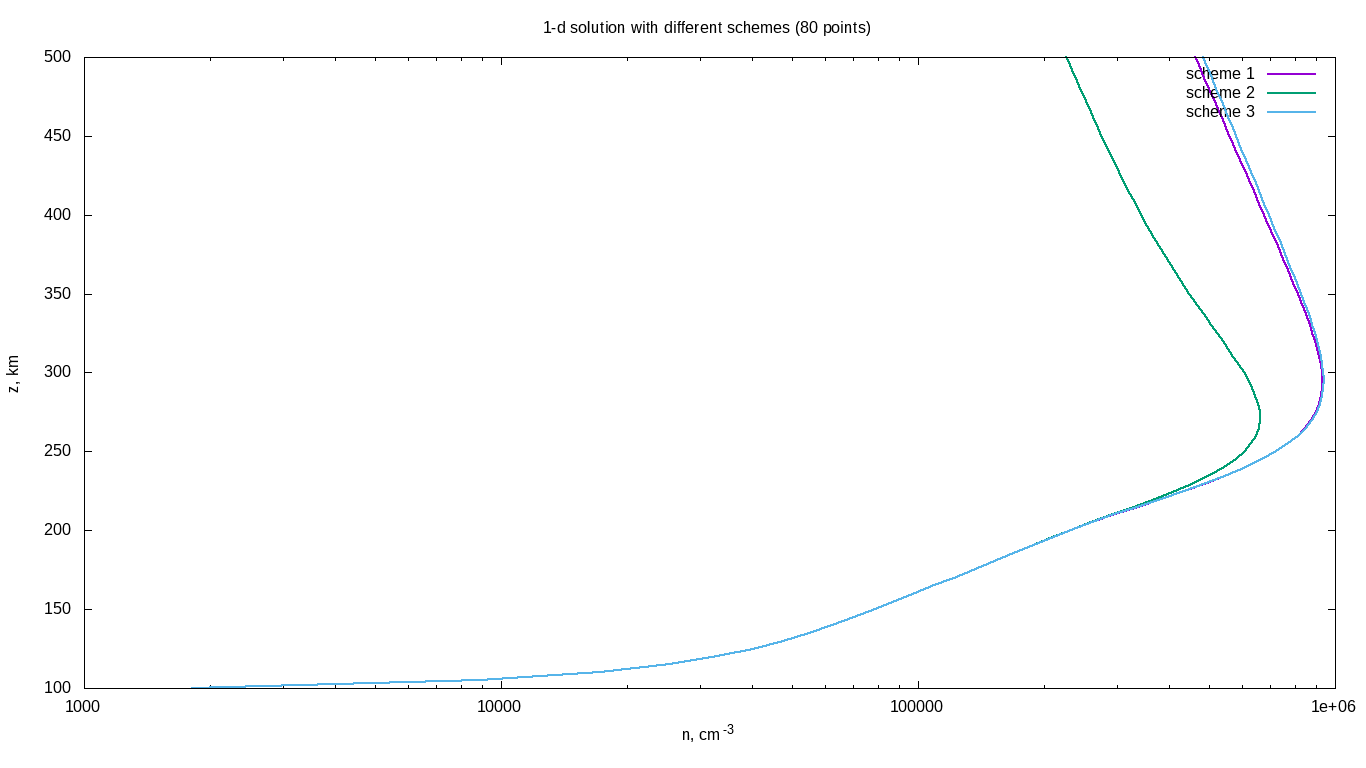
\includegraphics[scale=0.5]{1d_stationary_logscale_80}}
\caption{Стационарные решения на $80$ расчётных узлах.}
\end{figure}

\begin{figure}[H]
\center{
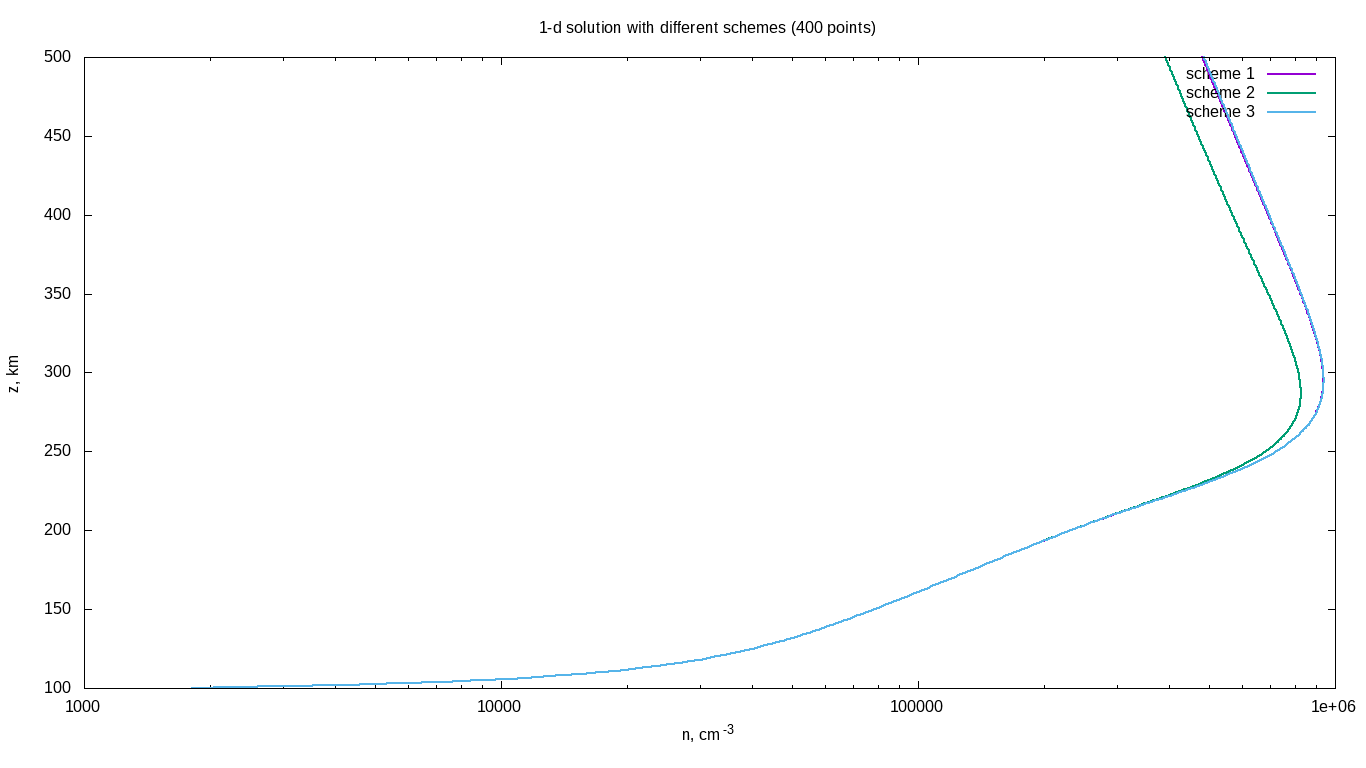
\includegraphics[scale=0.5]{1d_stationary_logscale_400}}
\caption{Стационарные решения на $400$ расчётных узлах.}
\end{figure}

\begin{figure}[H]
\center{
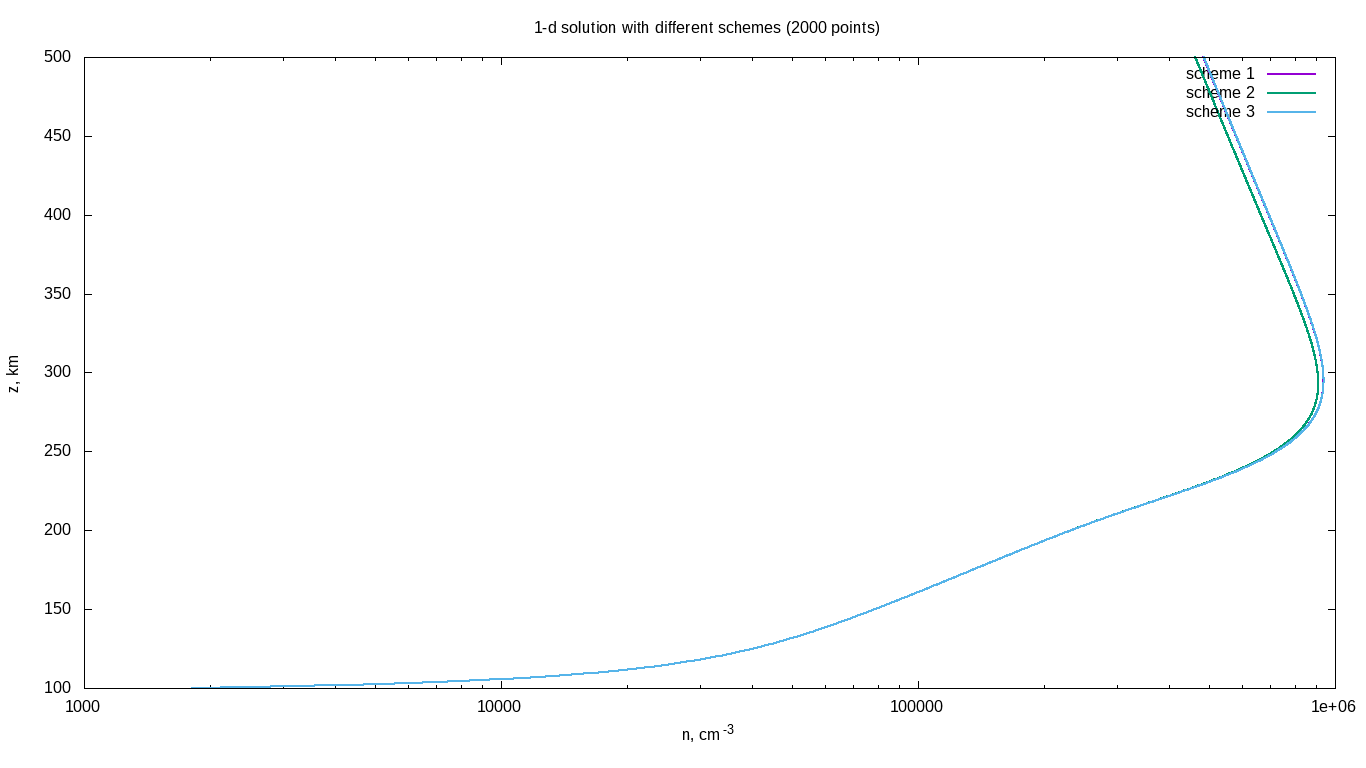
\includegraphics[scale=0.5]{1d_stationary_logscale_2000}}
\caption{Стационарные решения на $2000$ расчётных узлах.}
\end{figure}

Полученное решение позволяет исследовать чувствительность к изменению различных входящих в уравнение внешних параметров: температурам, концентрациям нейтральных молекул, фотоионизации и рекомбинации. На следующих ниже графиках представлены результаты варьирования каждого из параметров в отдельности на $10\%$ и $20\%$ (в обе стороны).

\medskip

Варьирование входящих в уравнение температур показывает, что наибольшую чувствительность решение имеет к температуре нейтральных молекул:


\begin{figure}
\center{
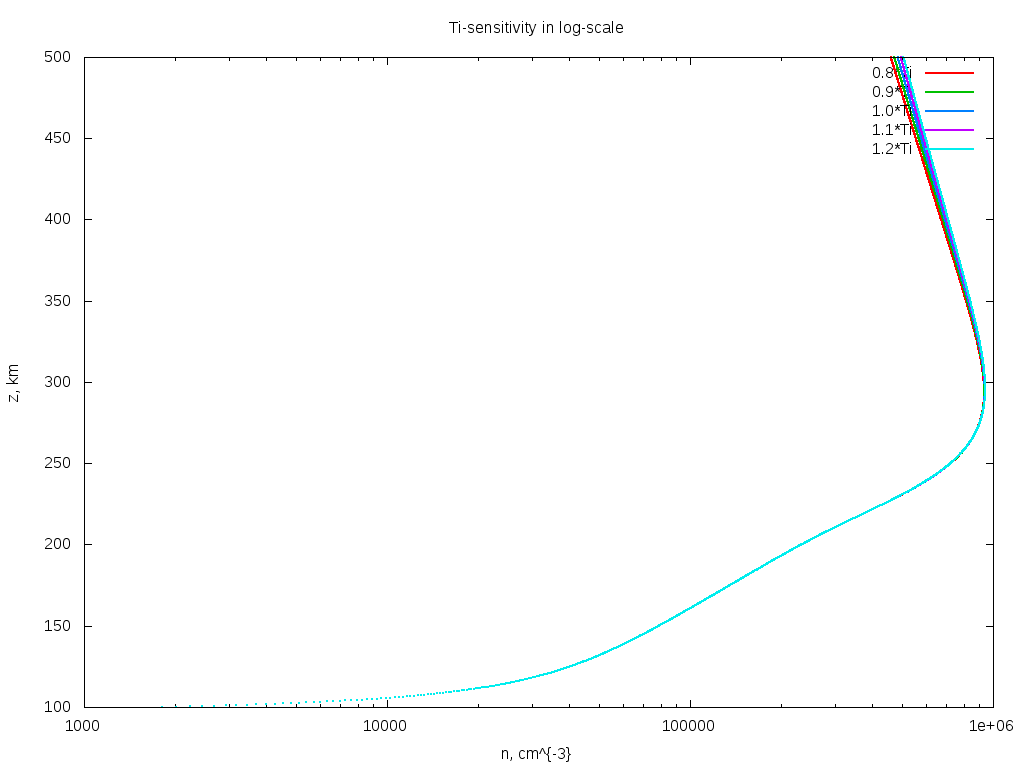
\includegraphics[scale=0.5]{Ti-sensitivity_log}}
\caption{Чувствительность к изменению температуры ионов.}
\end{figure}

\begin{figure}
\center{
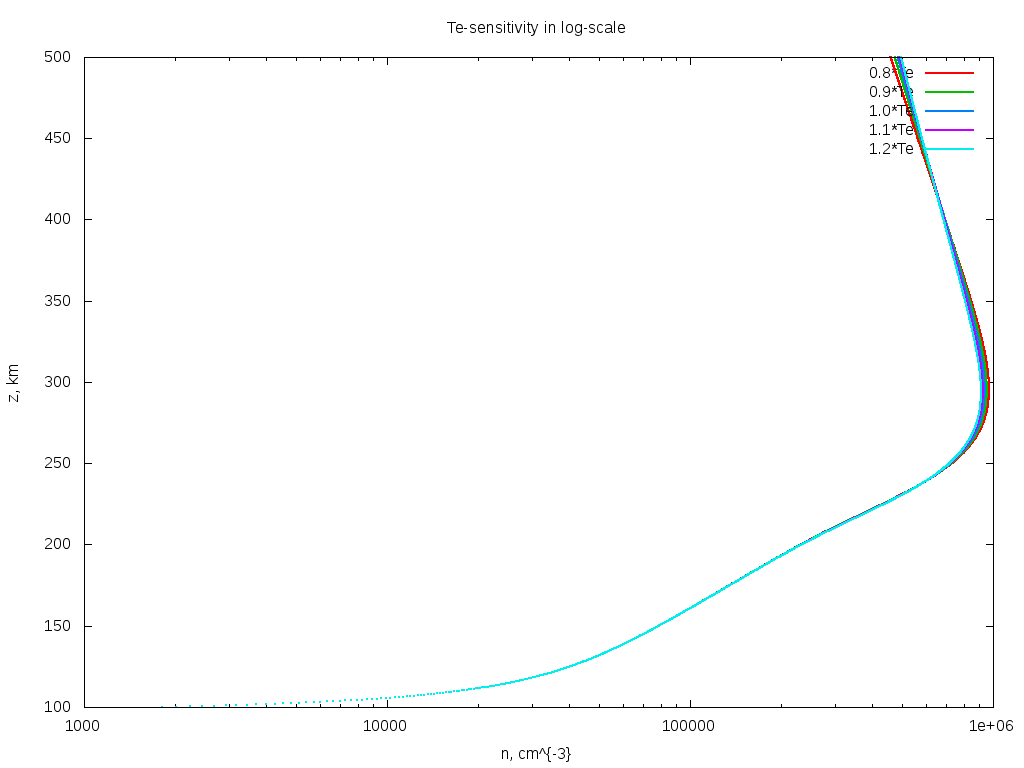
\includegraphics[scale=0.5]{Te-sensitivity_log}}
\caption{Чувствительность к изменению температуры электронов.}
\end{figure}

\begin{figure}
\center{
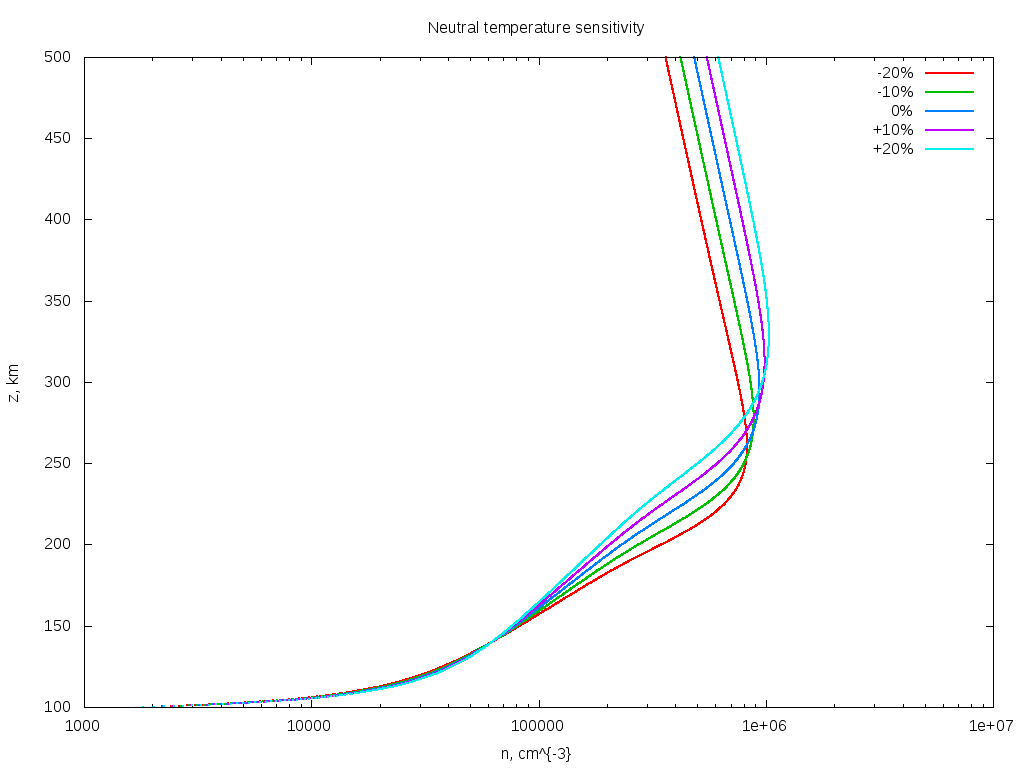
\includegraphics[scale=0.5]{Tn-sensitivity_log}}
\caption{Чувствительность к изменению температуры нейтральных молекул.}
\end{figure}

\medskip 

Теперь изменяем 








\end{document}





